%! Tex program = pdflatex
 
\documentclass[UTF8]{ctexart}
\CTEXsetup[format={\Large\bfseries}]{section}
\usepackage{amsmath}
\usepackage{ctex}
\usepackage{array}
\usepackage{ulem}
\usepackage{graphicx}
\usepackage{geometry}
\usepackage{multirow}
\usepackage{subfig}
\usepackage{float}
\usepackage{multicol}
\usepackage{multirow}
\usepackage{indentfirst}
\usepackage{makecell}
\geometry{papersize={21cm,29.7cm}}
\geometry{left=2.54cm,right=2.54cm,top=3.18cm,bottom=3.18cm}
\usepackage{fancyhdr}
\pagestyle{fancy}
\lhead{\today}
\chead{}
\rhead{2020011075}
\lfoot{清华大学}
\cfoot{\thepage}
\rfoot{物理实验B(1)}
\renewcommand{\headrulewidth}{0.4pt}
\renewcommand{\headwidth}{\textwidth}
\renewcommand{\footrulewidth}{0pt}
\usepackage{bm}
\begin{document}
\begin{titlepage}
    \begin{center}
		\quad \\
		\quad \\
        \quad \\
        \quad \\
        \quad \\
        \quad \\
		\kaishu \fontsize{30}{15} 准稳态测不良导体导热系数和比热

	\end{center}
	\vskip 10cm

    \begin{center}
        \begin{large}
        \begin{tabular}{cc}
        院\qquad 系:& ~~~~~~~~自动化系~~~~~~~~      \\
        \cline{2-2}\\
        班\qquad 级:& 自02班   \\
        \cline{2-2}\\
        学生姓名:& 彭程    \\
        \cline{2-2}\\
        学\qquad 号:&2020011075   \\
        \cline{2-2}\\
        组\qquad 号:& 单一晚M    \\
        \cline{2-2}\\
        座~~位~~号:& \# 13    \\
        \cline{2-2}
        \end{tabular}
        \end{large}
        \end{center}

\end{titlepage}
\newpage
\tableofcontents
\newpage
\section{实验名称}
准稳态测不良导体的导热系数和比热
\section{实验目的}
\begin{enumerate}
\item 了解准稳态法测不良导体的导热系数和比热的原理, 掌握其操作方法;
\item 掌握使用热电偶测量温度的方法;
\end{enumerate}
\section{实验原理}
    \subsection {热传导} 
    由傅里叶定律
    $$
    Q=-\lambda F \frac{\mathrm{d} t}{\mathrm{~d} x}
    $$
    
    可导出
    $$
    q=\frac{Q}{F}=-\lambda \frac{d t}{d x}
    $$

    其中q为热流密度,比例系数$\lambda$为材料的导热系数(热导率),符号表示热流方向与温度梯度方向相反。

    \subsection {一阶导热模型} 

    此次试验采用厚度为2R的无限大平板模型进行热导率测量,从板的两端面进行功率相同的均匀热流加热,则板内温度分布以中心截面对称。





    \subsection {热传导方程及解} 

    对应上述模型的一维导热方程:
    $$
    \frac{\partial t(x, \tau)}{\partial \tau}=a \frac{\partial^{2} t(x, \tau)}{\partial x^{2}}
    $$

    初始条件:
$$
\left.t(x, \tau)\right|_{\tau=0}=t_{0}
$$

    边界条件:
$$
\left.\lambda \frac{\partial t(x, \tau)}{\partial x}\right|_{x=R}=q_{c},\left.\frac{\partial t(x, \tau)}{\partial x}\right|_{x=0}=0
$$

    式中  0<x<R, $\tau>0$, $a=\frac{\lambda}{c \rho}$  为热扩散率,  c  与 $ \rho $ 分别为材料的比热与密度。

    利用分离变量法可以解出方程的解为:
    $$
    t(x, \tau)-t_{0}=\frac{q_{c}}{\lambda}\left[\frac{a \tau}{R}-\frac{R^{2}-3 x^{2}}{6 R}+R \sum_{n=1}^{\infty}(-1)^{n+1} \frac{2}{\mu_{n}^{2}} \cos \left(\mu_{n} \frac{x}{R}\right) \exp \left(-\mu_{n}^{2} F_{0}\right)\right]
    $$

    式中 $ \mu_{n}=n \pi, n=1,2,3, \ldots $

    $F_{0}=\frac{a \tau}{R^{2}}$  为傅里叶数 (无量纲),
    $ t_{0} $ 为初始温度

    经过一定时间, 当 $ F_{0}=\frac{a \tau}{R^{2}}>0.5 $ 时, 上式中的级数求和项变得很小, 可以化为:
    $$
    t(x, \tau)-t_{0}=\frac{q_{c} R}{\lambda}\left(\frac{a \tau}{R^{2}}+\frac{x^{2}}{2 R^{2}}-\frac{1}{6}\right)
    $$

    这种状态叫做准稳态,特点如下:
    
    (1) 样品表面和中心的温度差  $\Delta t=\frac{q_{\mathrm{e}} R}{2 \lambda}$  保持恒定。
    
    (2) 样品中心升温速率 $ \left.\frac{\partial t}{\partial \tau}\right|_{x=0}=\frac{q_{c a} a }{\lambda R}=\frac{q_{c}}{c \rho R} $ 保持恒定。
    
    据此, 通过测出温度差与升温速率即可测量不良导体的热导率 $ \lambda $ 和 热容  $c$  。

    \subsection {表面热流密度$q_c$的计算和温度差的测量} 
     本实验中温差使用热电偶测量。  当 热电偶两端T 和 $T_{0} $温度不等时, 回路中近似产生温差电动势  $U = k\left(T-T_{0}\right)$ 。  
    本实验中,  $k = 40 \mu V /{ }^{\circ} \mathrm{C}$  
 
    本实验中热源向两侧均匀散热, 故热流密度表达式为 $ q_{c} = \frac{U^{2}}{2 F r}$, U 为薄膜加热电压,  F  为薄膜面积,r为单个加热器的电阻。 

    \section{实验仪器}
    \noindent 样品台装置:

    平行板试样4块:有机玻璃,长宽90mm,厚度10mm
    
    薄膜加热器 2 片, 加热电压控制在  $15-19.9 \mathrm{~V}$  之间

    热电偶2只

    泡沫绝热体 2 块

    \noindent 函数信号发生器

    \noindent 数字万用表

    \noindent 直流稳压电源

    \noindent 保温杯 (冷端)

    \noindent 换向开关

    \noindent 秒表

    \noindent 电容、电阻、二极管

    \section{实验任务}
    \subsection{实验步骤} 

    \noindent  (1) 阅读说明书并练习数字万用表的使用, 测量交流电压有效值及频率、交流信号频率、 电阻值(二端法)、电容及二极管正向导通电压;\\
    
    \noindent  (2)完成样品台组装。打开直流稳压电源、数字万用表电源并预热一段时间, 在适当预 设电压下, 用万用表测量实验前加热电压;\\
    
    \noindent  (3)用万用表测量并记录热电偶、加热器电阻值, 检查器件是否完好;\\
    
    \noindent  (4)连接热电偶、换向开关与数字万用表, 组装测温系统, 将热电偶各接点摆放到位;\\
    
    \noindent  (5)使用温度计测量初始温度 $ t_{0} $ 及初始温差 $ U_{1}\left(t_{2} t_{1}\right)$  、初始中心面温度 $ U_{2}\left(t_{1} t_{c}\right) $ 。接通 电源与加热器, 间隔 1 分钟测量 $ U_{1}\left(t_{2} t_{1}\right)  $与 $ U_{2}\left(t_{1} t_{c}\right) $, 共测量约 25 分钟;\\
    
    \noindent  (6)断开电源并拆下万用表, 测量试验后的加热电压。进行数据处理。
    


\section{数据处理}

\subsection{万用表的使用练习}

\begin{tabular}{|c|c|c|c|c|c|}
\hline 测量任务 & 测量值 & 量程 & 精度 & 不确定度 & 完整测量结果 \\
\hline 电阻R &  $10.8458 \Omega$  &  $20 \mathrm{k} \Omega $ &  0.02+0.004  &  $0.0030 \mathrm{k} \Omega$  &  $(10.8458 \pm 0.0030) \mathrm{k} \Omega$  \\
\hline 电容C &  $0.967 \mu \mathrm{F}$  &  $2 \mu \mathrm{F} $ &  1+0.5  &  $0.0020 \mu \mathrm{F}$  &  $(0.967 \pm 0.0020) \mu \mathrm{F}$  \\
\hline 交流电压U & $ 0.39372 \mathrm{~V}$  & $ 2 \mathrm{~V} $ &  0.2+0.05  &  $0.0018 \mathrm{~V}$  &  $(0.3937 \pm 0.0018) \mathrm{V} $ \\
\hline 交流信号f &  $1000.00 \mathrm{Hz} $ &  $20 \mathrm{~Hz}-1 \mathrm{kHz} $ &  0.01+0.003  & $ 0.13 \mathrm{Hz}$  & $ (1000.00 \pm 0.13) \mathrm{Hz} $ \\
\hline 二极管导通电压 & \multicolumn{5}{|c|}{ 正向导通电压  $=0.5713 \mathrm{~V}$ }\\
\hline
\end{tabular}\\

\noindent 不确定度计算:

(1) 电阻R
$$
\delta =0.02 \% \times 10.8458+0.004 \% \times 20=0.0030 \Omega
$$

(2) 电容C
$$
\delta  =1 \% \times 0.967+0.5 \% \times 2=0.0020 \mu F
$$

(3) 交流电压U
$$
\delta =0.2 \% \times 0.39373+0.05 \% \times 2=0.0018 V
$$

(4) 交流信号f
$$
\delta =0.01 \% \times 1000.00+0.003 \% \times 1000 =0.13 Hz
$$




\subsection{热导实验准备、器件检查}

\noindent 1.热电偶\\

\begin{tabular}{|c|c|c|c|}
\hline 中心面热电偶阻值  / $\Omega$  & 加热面热电偶阻值  /$ \Omega $ & 中心面冷端热电偶阻值  /$ \Omega $ & 加热面冷端热电偶阻值  /$ \Omega $ \\
\hline $ 3.335 \Omega$  &  $2.556\Omega$  &  $3.610 \Omega $ &  $3.658 \Omega$  \\
\hline
\end{tabular}\\

\noindent 2.加热薄膜并联阻值$= 55.200\Omega $\\

\noindent 3.冷端水温(室温)$= 20.7^\circ C $\\

\noindent 4.初始加热电压=17.9987 V ,  结束加热电压=17.9988 V ,平均加热电压=17.9988V   


\subsection{温差电动势测量数据}


\begin{tabular}{|c|c|c|c|c|c|c|c|c|c|}
    \hline $\tau(\min )$ & 0 & 1 & 2 & 3 & 4 & 5 & 6 & 7 & 8 \\
    \hline $\text { 中心面 } U_2\left(t_{1} t_{c}\right) / m V$ & 0.004 & 0.006 & 0.011 & 0.025 & 0.043 & 0.061 & 0.092 & 0.106 & 0.129 \\
    \hline $\text { 加热面 } U_1\left(t_{2} t_{1}\right) / m V$ & 0.003 & 0.106 & 0.144 & 0.168 & 0.175 & 0.184 & 0.189 & 0.193 & 0.193 \\
    \hline $\tau(\min )$ & 9 & 10 & 11 & 12 & 13 & 14 & 15 & 16 & 17 \\
    \hline $\text { 中心面 } U_2\left(t_{1} t_{c}\right) / m V$ & 0.149 & 0.173 & 0.196 & 0.218 & 0.243 & 0.265 & 0.288 & 0.311 & 0.334 \\
    \hline $\text { 加热面 } U_1\left(t_{2} t_{1}\right) / m V$ & 0.193 & 0.193 & 0.193 & 0.193 & 0.193 & 0.193 & 0.193 & 0.193 & 0.193 \\
    \hline $\tau(\min )$ & 18 & 19 & 20 & 21 & 22 & 23 & 24 & 25 & \\
    \hline $\text { 中心面 } U_2\left(t_{1} t_{c}\right) / m V$ & 0.357 & 0.380 & 0.402 & 0.425 & 0.448 & 0.470 & 0.492 & 0.514 & \\
    \hline $\text { 加热面 } U_1\left(t_{2} t_{1}\right) / m V$ & 0.193 & 0.192 & 0.192 & 0.191 & 0.191 & 0.191 & 0.190 & 0.190 & \\
    \hline
\end{tabular}



\begin{figure}[H]
    \centering
    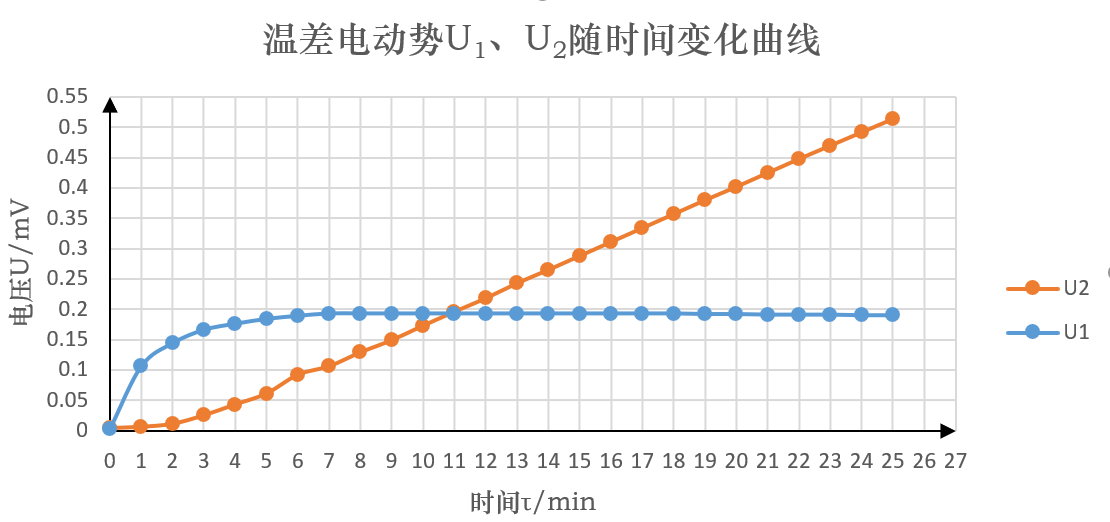
\includegraphics[scale=0.8]{绘图.png}
    \caption{$U_1$、$U_2$随时间变化曲线}
    \label{fig:label}
\end{figure}

\begin{figure}[H]
    \centering
    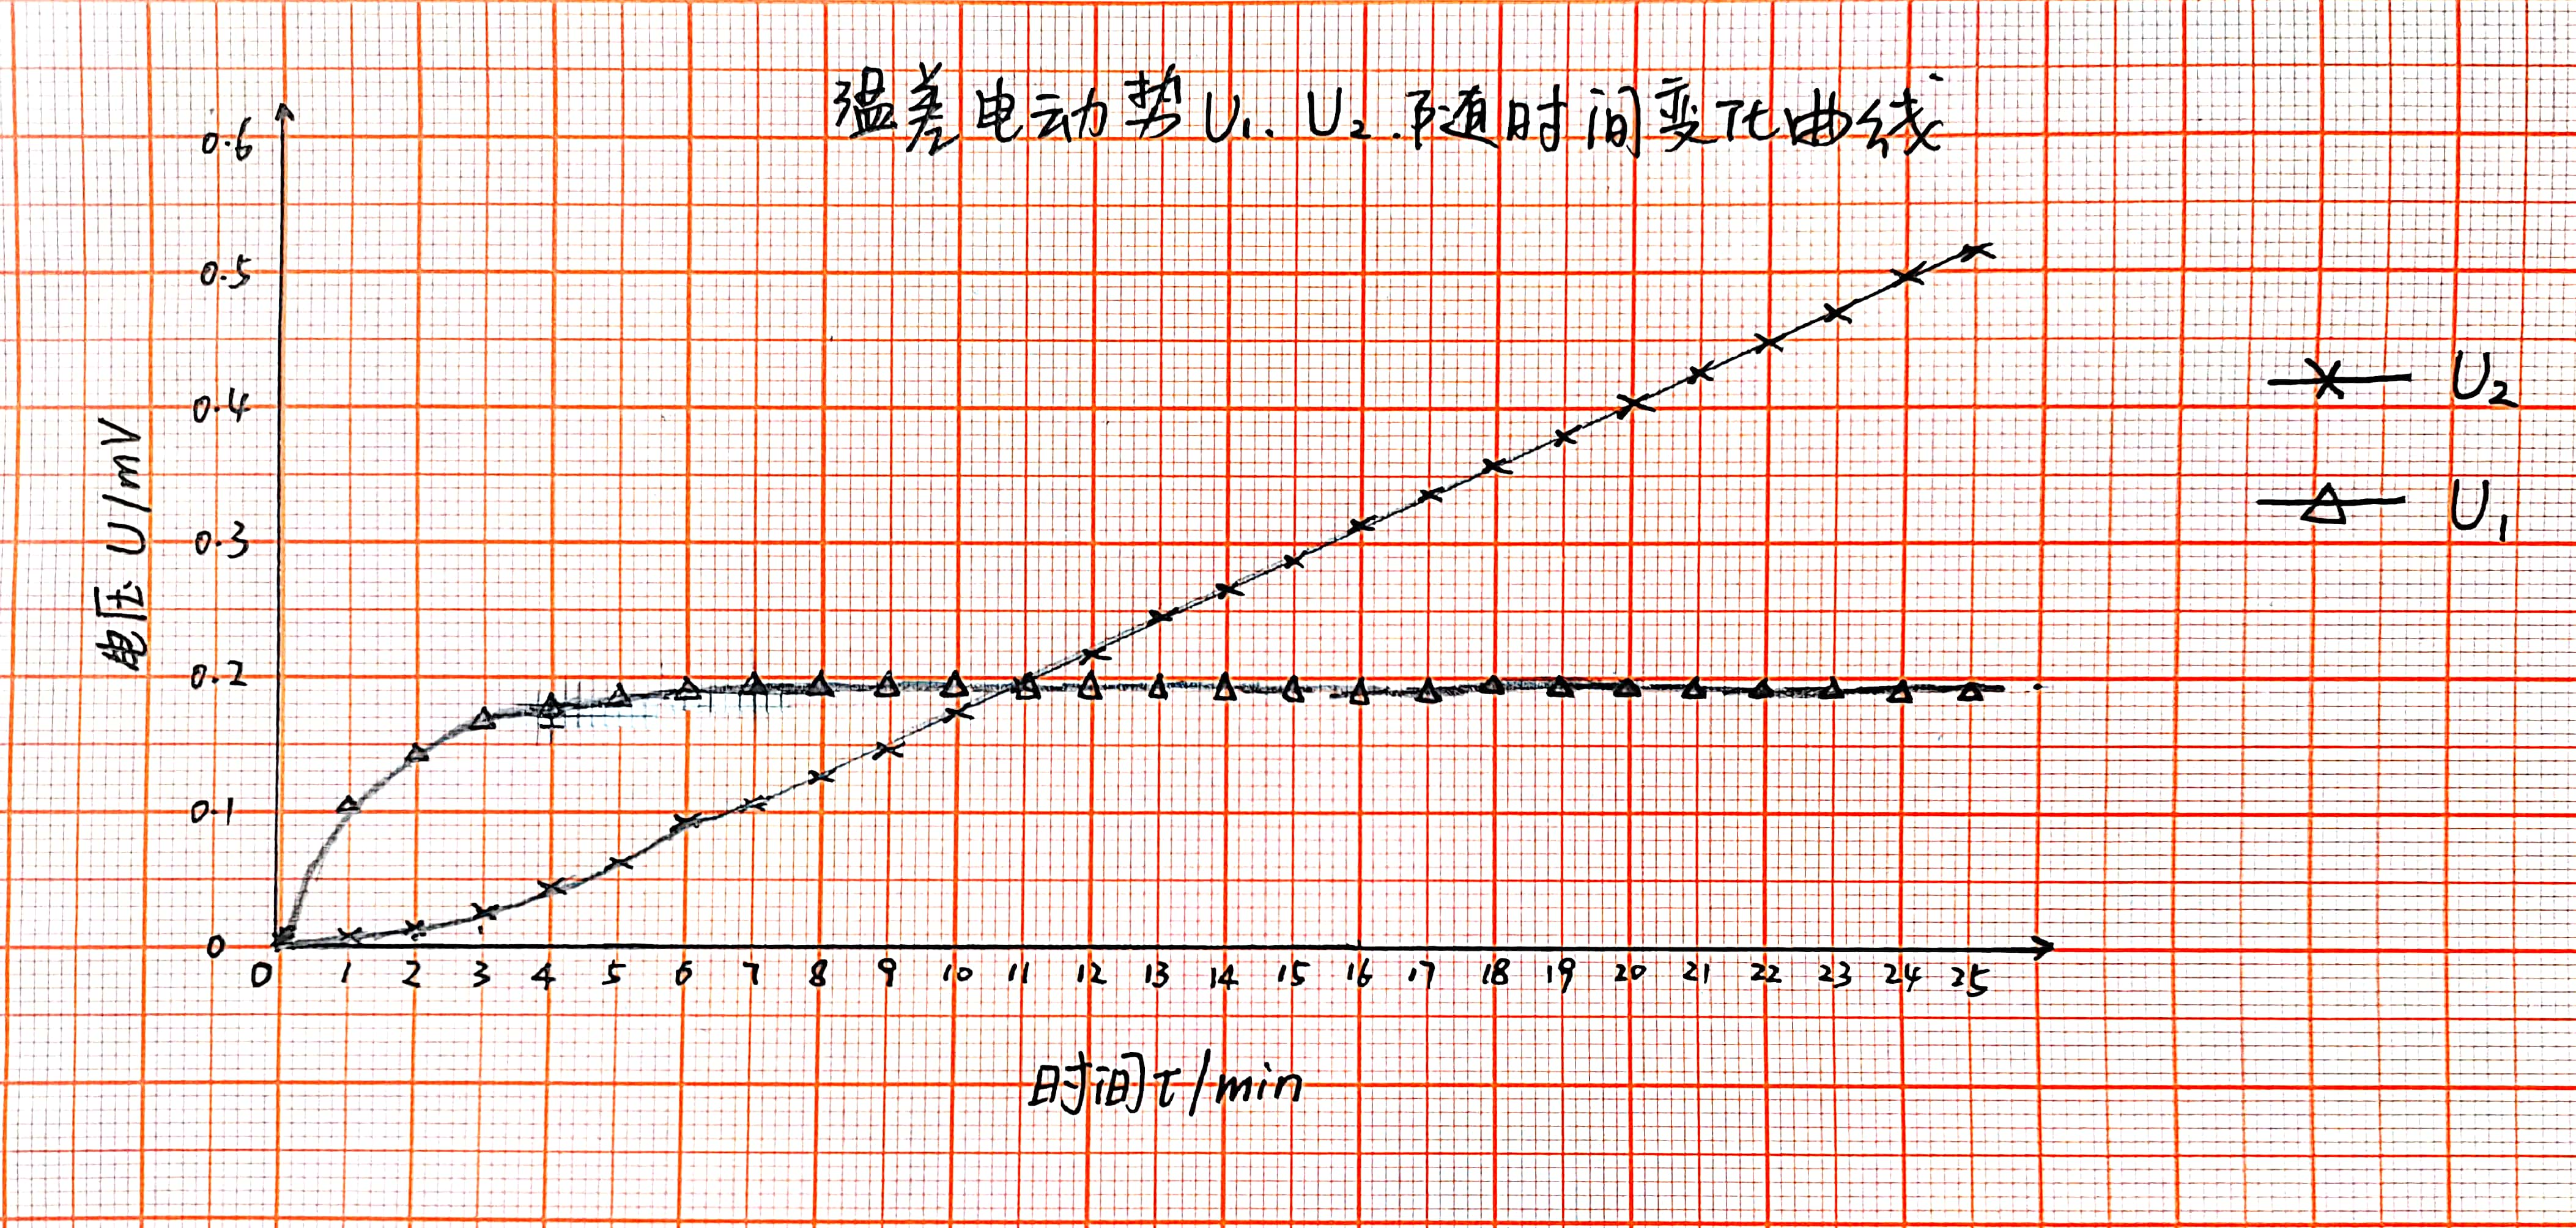
\includegraphics[scale=0.09]{手绘波形.jpg}
    \caption{$U_1$、$U_2$随时间变化曲线手绘图}
    \label{fig:label}
\end{figure}



从图线中可看出, 大约在第 $ 7 \min $ 后, $ U_{1}\left(t_{2}, t_{1}\right)$  加热面与中心面的温差不再发生变化, 可以认为进入 准稳态状态。

在准稳态下, 计算加热面与中心面的温差:
$$
\Delta t=\frac{U_{1}\left(t_{2} ,t_{1}\right)}{k}=\frac{193 \mu V}{40 \mu V /{ }^{\circ} \mathrm{C}}=4.825^{\circ} \mathrm{C}
$$

计算热流密度:
$$
q_{c}=\frac{U^{2}}{2 F r}=\frac{17.9988^{2}}{2 \times 0.09^{2} \times 2\times 55.200 }=181.140 \mathrm{~W} / \mathrm{m}^{2}
$$

因此, 导热系数 $ \lambda$  计算结果为: (样品厚度  $R=10 \mathrm{~mm} $ )
$$
\lambda=\frac{q_{c} R}{2 \Delta t}=\frac{181.14\times 0.01}{2\times 4.825}=0.188 W /(m \cdot K)
$$


对7min后$U_2$的图像进行线性拟合,
拟合图像如下:

\begin{figure}[H]
    \centering
    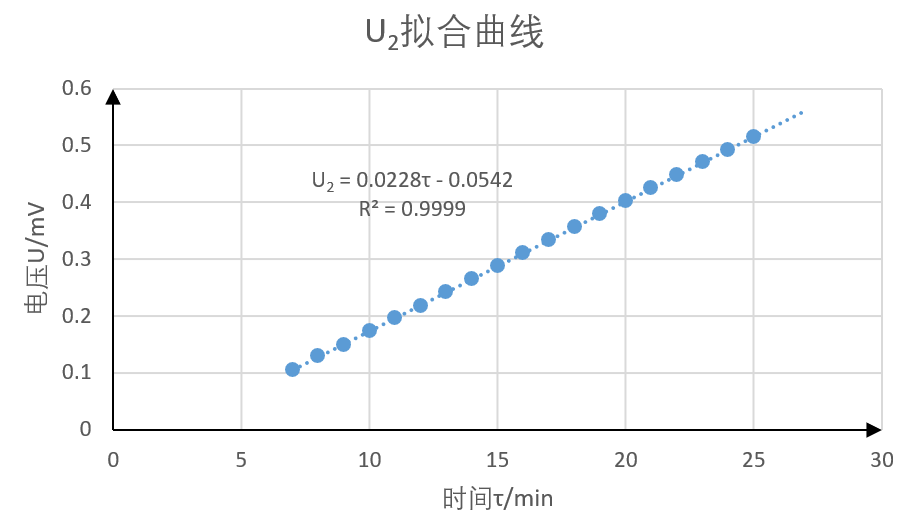
\includegraphics[scale=0.8]{拟合曲线.png}
\end{figure}






由线性拟合结果可得:

$$
\frac{\mathrm{d} U_{2}\left(t_{1} ,t_{c}\right)}{\mathrm{d} \tau}=0.0228 \mathrm{mV} / \min
$$

$$
\frac{\mathrm{d} t}{\mathrm{~d} \tau}=\frac{1}{k} \frac{\mathrm{d} U_{2}}{\mathrm{~d} \tau}=0.570^{\circ} \mathrm{C} / \min =9.50 \times 10^{-3 \circ} \mathrm{C} / \mathrm{s}
$$

因此, 比热  c  计算结果为: $\left(\rho=1196 \mathrm{~kg} / \mathrm{m}^{3}, q_{c}=181.37 \mathrm{~W} / \mathrm{m}^{2}\right) $

$$
c=\frac{q_{c}}{\rho R \frac{\mathrm{dt}}{\mathrm{dr}}}=1.594 \times 10^{3} \mathrm{~J} /(\mathrm{kg} \cdot K)
$$


 

 若认为$\tau = 7 \mathrm{~min}$  时进入准稳态, 取 $ U_{2}\left(t_{1}, t_{c}\right) = 0.106 \mathrm{mV} $
 温差 $ t_{1} t_{c} = \frac{U_{2}\left(t_{1} t_{c}\right)}{k} = \frac{0.106}{0.04} = 2.65^{\circ} \mathrm{C} $,
 考虑到室温 $ t_{0} = t_{c} = 20.7^{\circ} \mathrm{C} $,
 故进入准稳态时, 中心面 $ t_{1} = 20.7+2.65 = 23.35^{\circ} \mathrm{C} $

 样品内各点温升速率相同且恒定, 任意两点之间温差不随时间改变, 故加热面与中心面温差不变, 
$U_{1}\left(t_{2} ,t_{1}\right) $ 保持稳定。  
 根据理论分析, 中心面的温升速率 $ \frac{\partial t}{\partial \tau} = \frac{q_{c}}{c \rho R} $保持不变, 故 $U_{2} (t_{1}, t_{c}) $ 与  $\tau$  呈线性关系。  
 
 若将热流密度按照电功率的  85 \%  修正, 则:

$$
q_{c}=85 \% \cdot \frac{U^{2}}{2 F r}=153.97 W / m^{2} 
$$
$$
 \lambda=\frac{q_{c} R}{2 \Delta t}=0.160 W /(m \cdot K)
$$
$$
 c=\frac{q_{c}}{\rho R \frac{\mathrm{d} t}{\mathrm{~d} \tau}}=1.355 \times 10^{3} J /(k g \cdot K)
$$


\section{实验总结}

通过本次实验,我学会了准稳态发测不良导体的导热系数和比热,明白了其背后原理,
实践了其操作方法,对于稳态、准稳态、瞬时测导热系数的原理方法有了较为全面的认识。
同时还掌握了热电偶测量温度的原理和接线方法。

由于之情的实验经历和专业上电子实验较多,所以对信号发生器和万用表较为熟悉,所以总体而言本次试验完成的比较顺利,没有遇到太多困难。
唯一的问题就是实验前对导热的设备不是太熟悉,导致在接线上出现了一些错误,不过后来及时改正了错误。
以后的实验中, 需要对仪器设备、 测量原理等充分熟悉。 科学实验
离不开严谨, 这应是贯穿操作始终的。

这是本学期最后一次物理实验,在这门课上我收获了很多,最后感谢助教的悉心指导!

(原始记录见尾页)

\section{原始实验数据}

\begin{figure}[H]
    \centering
    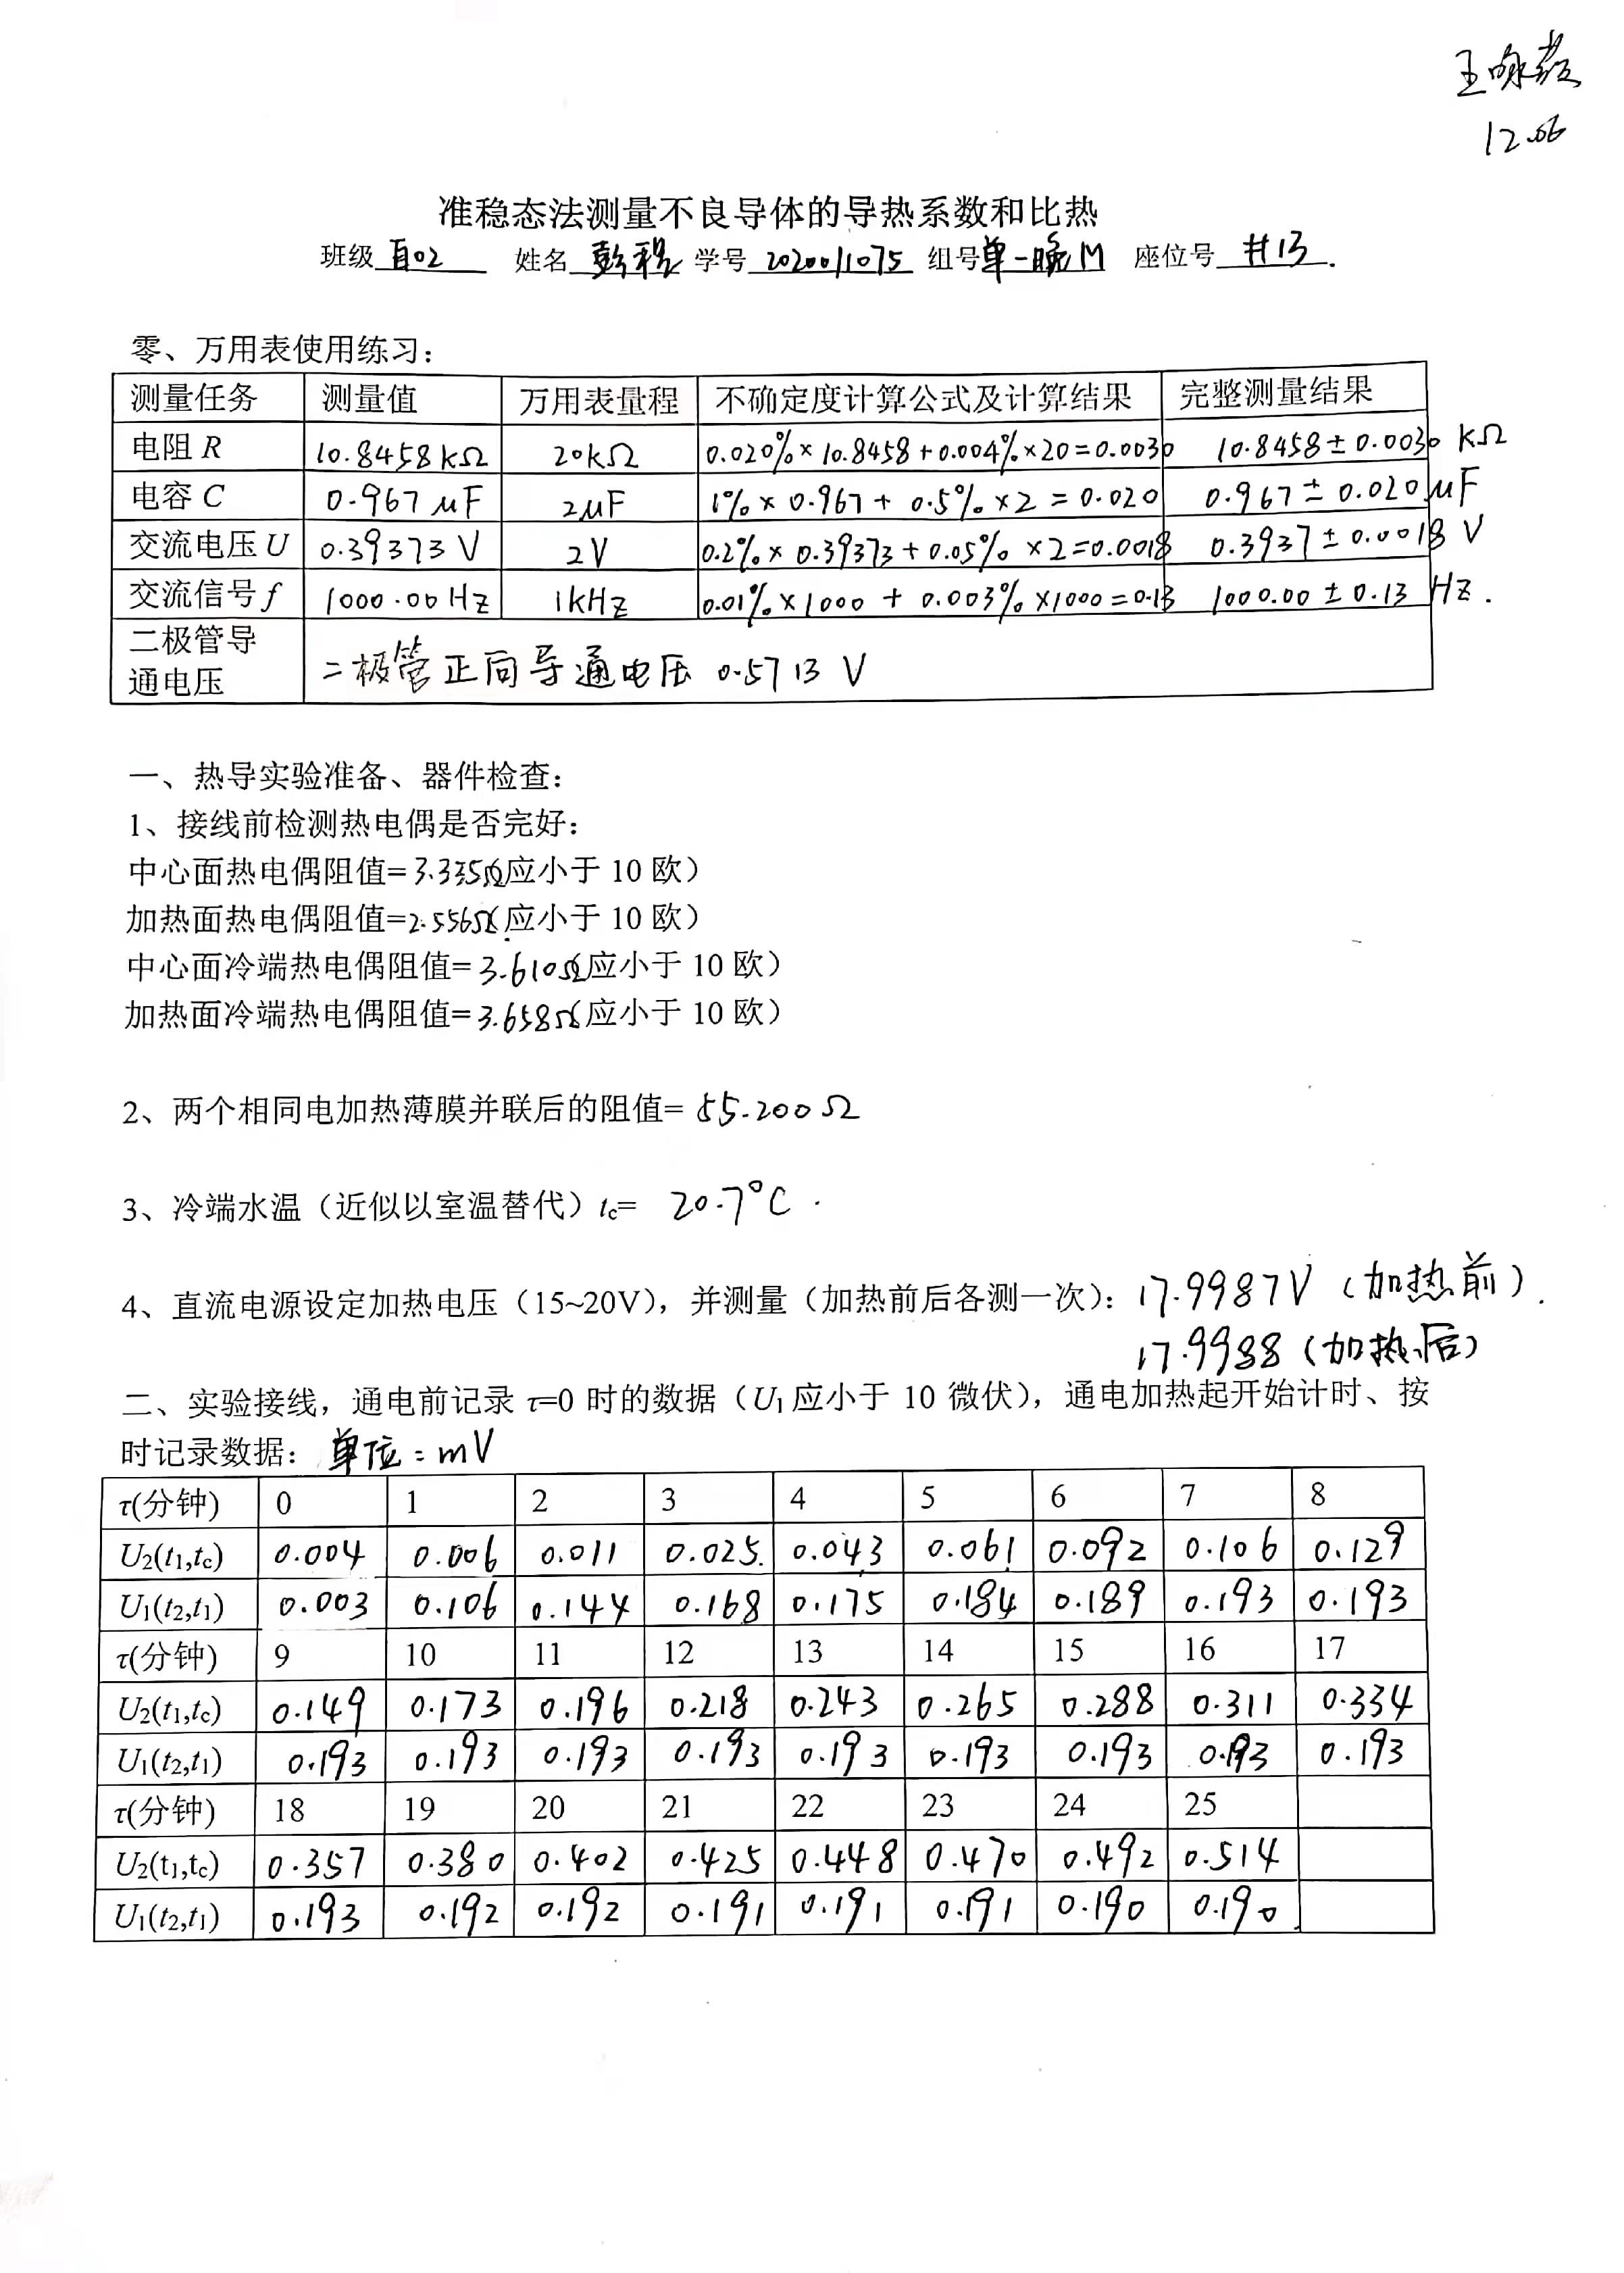
\includegraphics[scale=0.18]{原始记录.jpg}
\end{figure}

\end{document}